\documentclass[11pt]{article}
\usepackage[russian]{babel}
\makeatletter
\newcommand{\skipitems}[1]{%
	\addtocounter{\@enumctr}{#1}%
}
\makeatother

\newcommand{\numpy}{{\tt numpy}}
\usepackage{amsfonts}
\usepackage{amsmath}
\usepackage{graphics}
\usepackage{amsthm,amstext,amsfonts,bm,amssymb}
\usepackage{graphicx}
\usepackage{indentfirst}
\usepackage{subfigure}
\setlength{\parindent}{5ex}
\setlength{\parskip}{1em}
\usepackage[utf8x]{inputenc} 

\topmargin -.5in
\textheight 9in
\oddsidemargin -.25in
\evensidemargin -.25in
\textwidth 7in


\begin{document}
	
	\author{Биктимиров Данила Рустемович, ФКН}
	\title{Вариант 2}
	\date{}
	\maketitle
	
	\medskip
	
	\begin{enumerate}
		\item $$\begin{cases}
			\frac{dx}{dt} = -20x+5y = P(x,y)\\
			\frac{dy}{dt} = -120x+y = Q(x,y)
		\end{cases}$$
		
		Найдем особые точки: $$\begin{cases}
			-20x+5y = 0\\
			-120x+y = 0
		\end{cases}\Rightarrow\begin{cases}
			x = \frac{1}{4} y\\
			y = 120x
		\end{cases}\Rightarrow\begin{cases}
			x_0 = 0\\
			y_0 = 0
		\end{cases}$$
		
		$(0; 0)$ -- особая точка (критическая). Далее исследуем на устойчивость:
		$$ x = x_0 + \varepsilon, \:\: y = y_0 + \mu$$
		$$\begin{cases}
			\frac{d(\varepsilon)}{d(t)} = -20\varepsilon+5\mu\\
			\frac{d(\mu)}{d(t)} = -120\varepsilon+\mu 
		\end{cases}\Rightarrow \begin{vmatrix}
			-20-\lambda & 5\\
			-120 & 1 - \lambda
		\end{vmatrix} = 0$$
		$$ (-20-\lambda)(1-\lambda)- (-120)\cdot 5 =0 $$
		$$ \lambda ^2 + 19 \lambda + 580 = 0 $$
		$$ \lambda = -\frac{19}{2} \pm \frac{ i \sqrt{1959}}{2} $$
		
		Так как это два комплексных корня, и $Re  \lambda < 0$ получаем,что это устойчивый фокус.
		\begin{figure}[htbp!]
			\centering
			\subfigure[]
			{
				\begin{minipage}[b]{.3\linewidth}
					\centering
					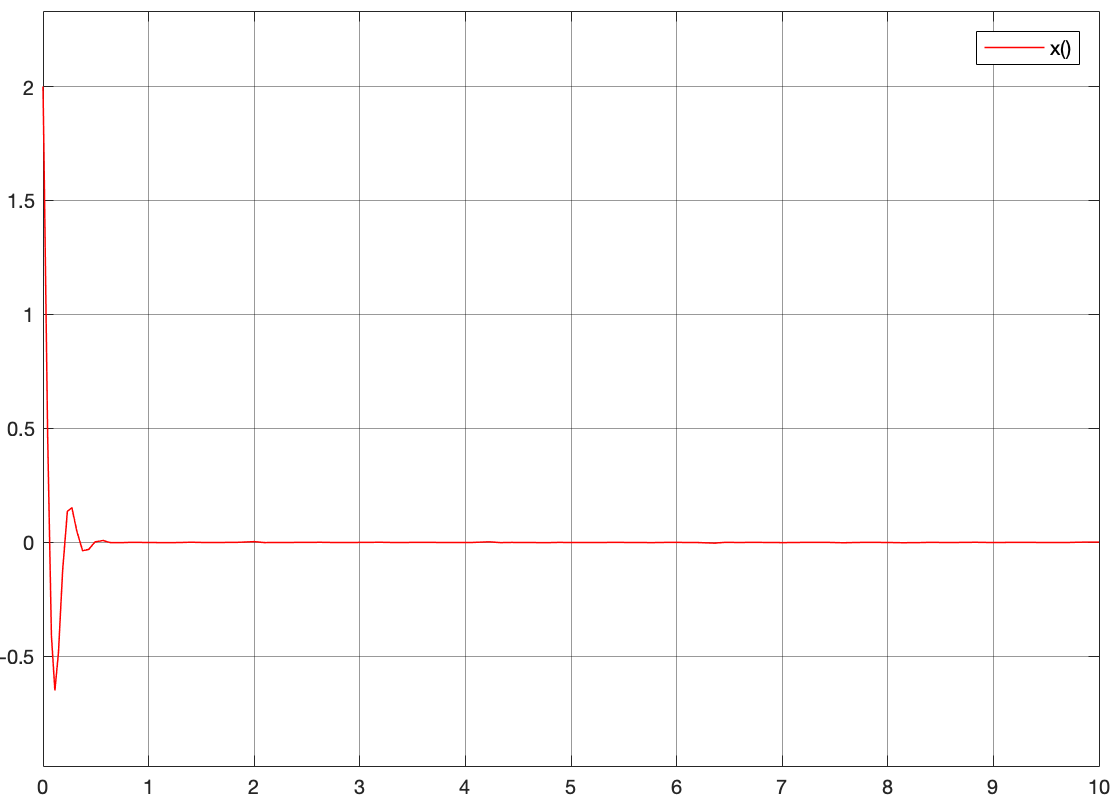
\includegraphics[scale=0.1]{x_1.png}
				\end{minipage}
				\begin{minipage}[b]{.3\linewidth}
					\centering
					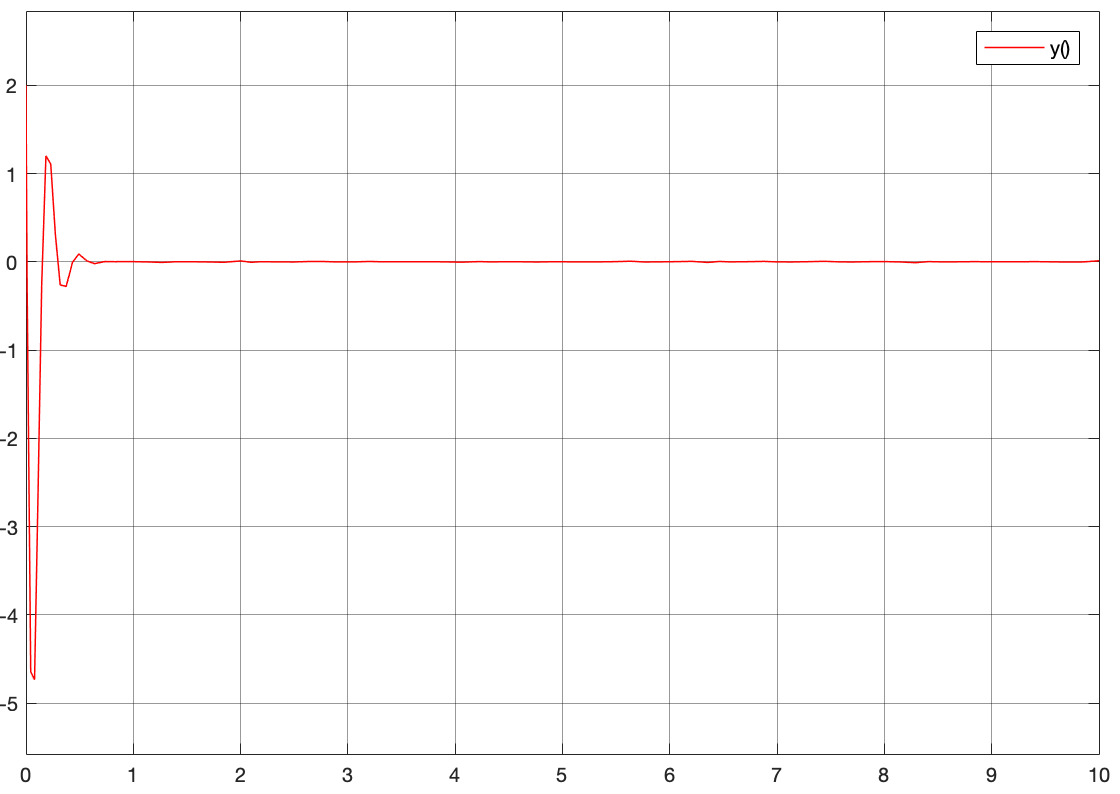
\includegraphics[scale=0.1]{y_1.png}
				\end{minipage}
			}
			\subfigure[]
			{
				\begin{minipage}[b]{.3\linewidth}
					\centering
					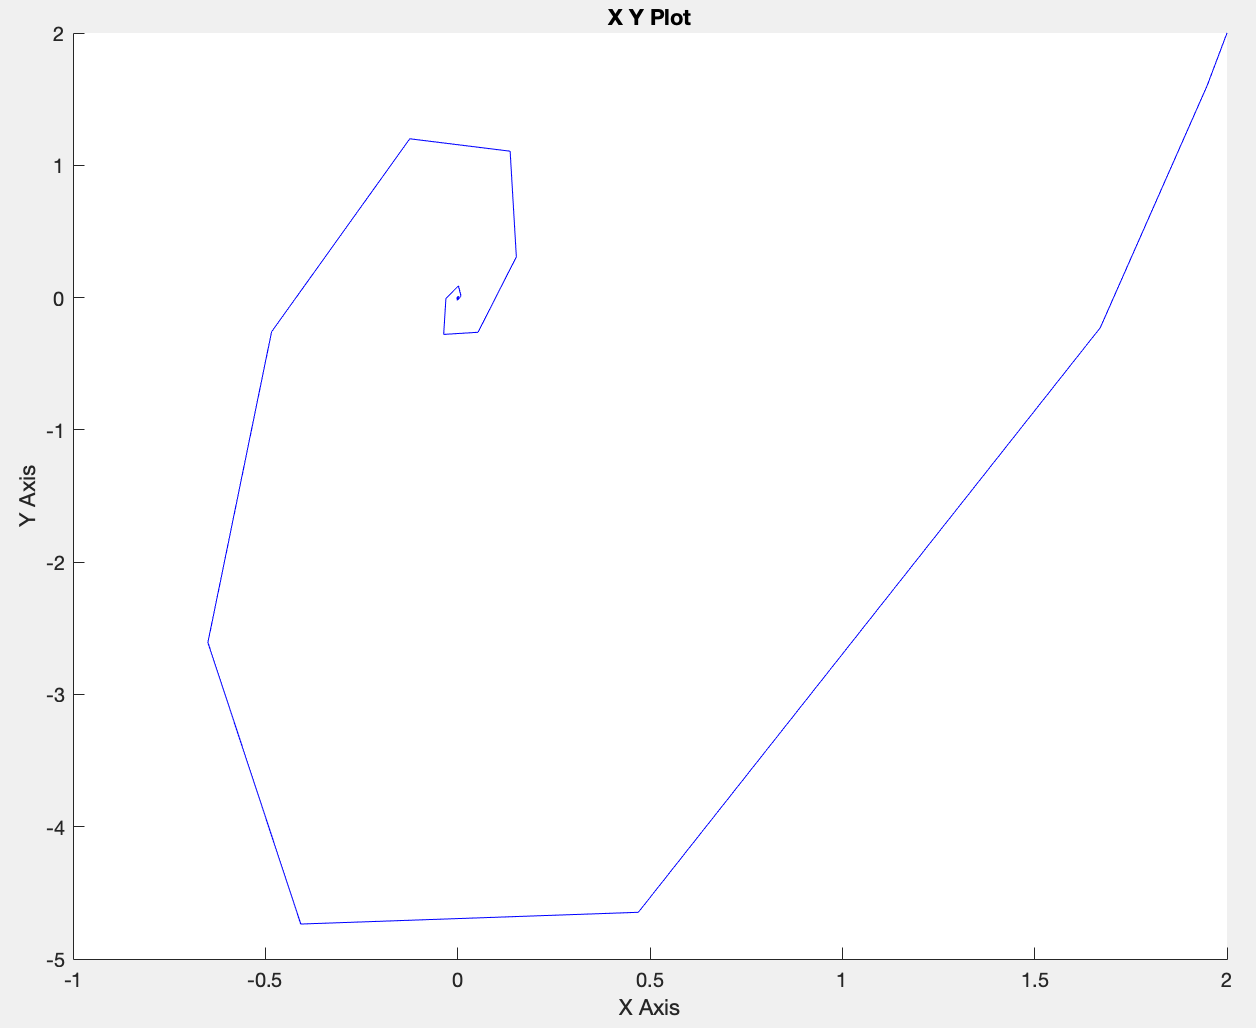
\includegraphics[scale=0.2]{xy.png}
				\end{minipage}
			}
			\caption{Кинетические (a) и фазовый (b) портреты при начальном значении $(x_0,y_0)=(2,2)$}
		\end{figure}
		\begin{figure}[ht!]
			\center{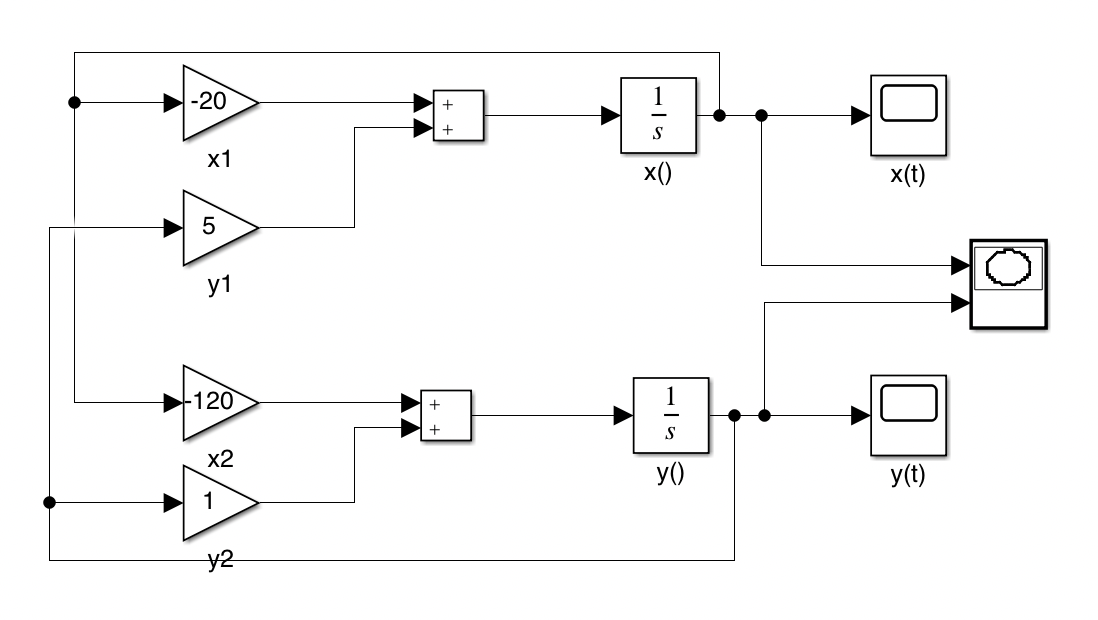
\includegraphics[scale=0.5]{model1.png}}
			\caption{Схема модели системы уравнений}
			\label{fig:image1}
		\end{figure}
		
		$$ $$
		\item $$
		\begin{cases}
			\frac{dx}{dt} = 3x-2xy-x^2 \\
			\frac{dy}{dt} = 2y - 2xy - y^2 + 3x^2
		\end{cases}
		$$
		\begin{enumerate}
			\item
			Ищем особые точки
			$$
			\begin{cases}
				3x-2xy-x^2 = 0 \\
				2y - 2xy - y^2 + 3x^2 = 0
			\end{cases}
			$$ 
			
			Заметим, что $x = 0$,  $y = 0$ является решением. Таким образом, точка $A(0;0)$ является критической. 
			
			При $x = 0$ система принимает вид:
			$$
			\begin{cases}
				0 = 0 \\
				2y - y^2  = 0
			\end{cases}
			\Leftrightarrow
			\begin{gathered}
				y = 0 \\
				y = 2 
			\end{gathered}
			$$ 
			
			Таким образом получаем критическую точку $B(0;2)$. 
			$$
			\begin{cases}
				3x-2xy-x^2 = 0 \\
				2y - 2xy - y^2 + 3x^2 = 0
			\end{cases}
			\Leftrightarrow
			\begin{cases}
				x(3-2y-x) = 0 \\
				2y - 2xy - y^2 + 3x^2 = 0
			\end{cases}
			\Leftrightarrow
			\begin{cases}
				y = \frac{3-x}{2} \\
				2y - 2xy - y^2 + 3x^2 = 0
			\end{cases}
			$$ 
			
			$$
			2\cdot\frac{3-x}{2} - 2x\cdot\frac{3-x}{2} - \left(\frac{3-x}{2}\right)^2 + 3x^2 = 0
			$$ 
			
			$$
			12-4x -12x+4x^2 - 9+6x-x^2 + 12x^2 = 0
			$$ 
			
			$$
			15x^2-10x+3=0 \Leftrightarrow
			\begin{gathered}
				x = \frac{\sqrt{5}-2i}{3\sqrt{5}} \\
				x = \frac{\sqrt{5}+2i}{3\sqrt{5}} 
			\end{gathered}
			$$ 
			
			Так получаем точки $C(\frac{\sqrt{5}-2i}{3\sqrt{5}}, \frac{4\sqrt{5}+i}{3\sqrt{5}})$ и $D(\frac{\sqrt{5}+2i}{3\sqrt{5}} , \frac{4\sqrt{5}-i}{3\sqrt{5}})$. 
			
			\item
			Исследование на устойчивость (рассматриваем только вещественные точки). $$ x = x_0 + \varepsilon, \:\: y = y_0 + \mu$$
			$$\begin{cases}
				\frac{d(\varepsilon)}{d(t)} = (3-2y-2x)\varepsilon+(-2x)\mu\\
				\frac{d(\mu)}{d(t)} = (-2y+6x)\varepsilon+(2-2x-2y)\mu 
			\end{cases}$$
			\begin{enumerate}
				\item $A(0;0)$
				$$\begin{cases}
					\frac{d(\varepsilon)}{d(t)} = (3)\varepsilon+(0)\mu\\
					\frac{d(\mu)}{d(t)} = (0)\varepsilon+(2)\mu 
				\end{cases}\Rightarrow \begin{vmatrix}
				3-\lambda & 0\\
				0 & 2 - \lambda
			\end{vmatrix} = 0$$
				$$ (3-\lambda)(2-\lambda) = 0$$
		
		Два положительных вещественных корня $\Rightarrow$ это неустойчивый узел.
				\item $B(0;2)$
				$$\begin{cases}
					\frac{d(\varepsilon)}{d(t)} = (-1)\varepsilon+(0)\mu\\
					\frac{d(\mu)}{d(t)} = (-4)\varepsilon+(-2)\mu 
				\end{cases}\Rightarrow \begin{vmatrix}
				-1-\lambda & 0\\
				-4 & -2 - \lambda
			\end{vmatrix} = 0$$
				$$ (-1-\lambda)(-2-\lambda) = 0$$
				Два отрицательных вещественных корня $\Rightarrow$ это устойчивый узел.
			\end{enumerate}

			
		\end{enumerate}
		\begin{figure}[htbp!]
			\centering
			\subfigure[$x(t),y(t)$]
			{
				\begin{minipage}[b]{.3\linewidth}
					\centering
					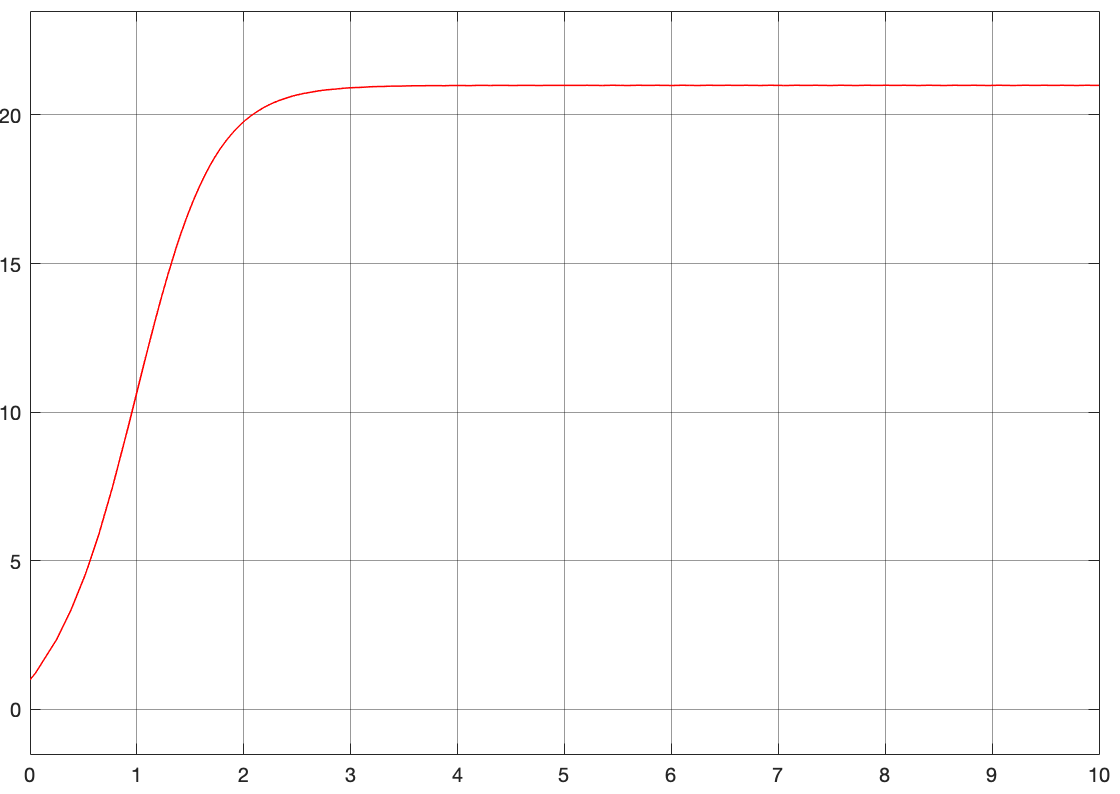
\includegraphics[scale=0.1]{x_2_11.png}
				\end{minipage}
				\begin{minipage}[b]{.3\linewidth}
					\centering
					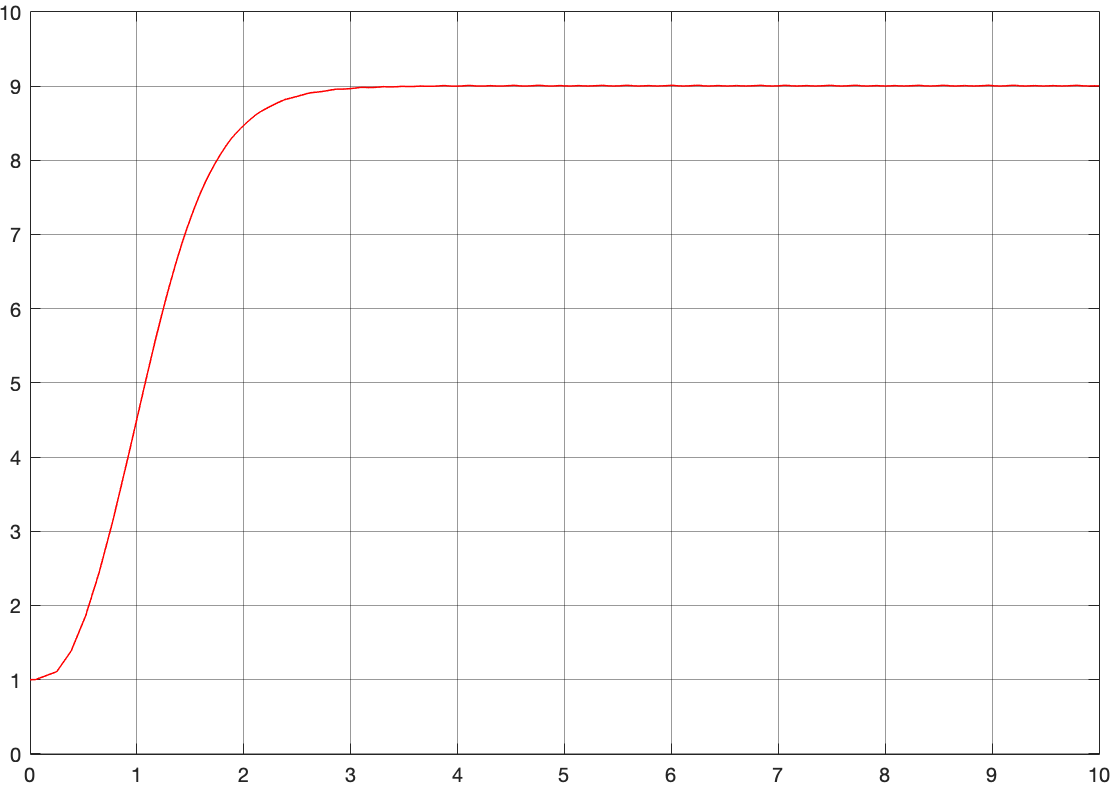
\includegraphics[scale=0.1]{y_2_11.png}
				\end{minipage}
			}
			\subfigure[]
			{
				\begin{minipage}[b]{.3\linewidth}
					\centering
					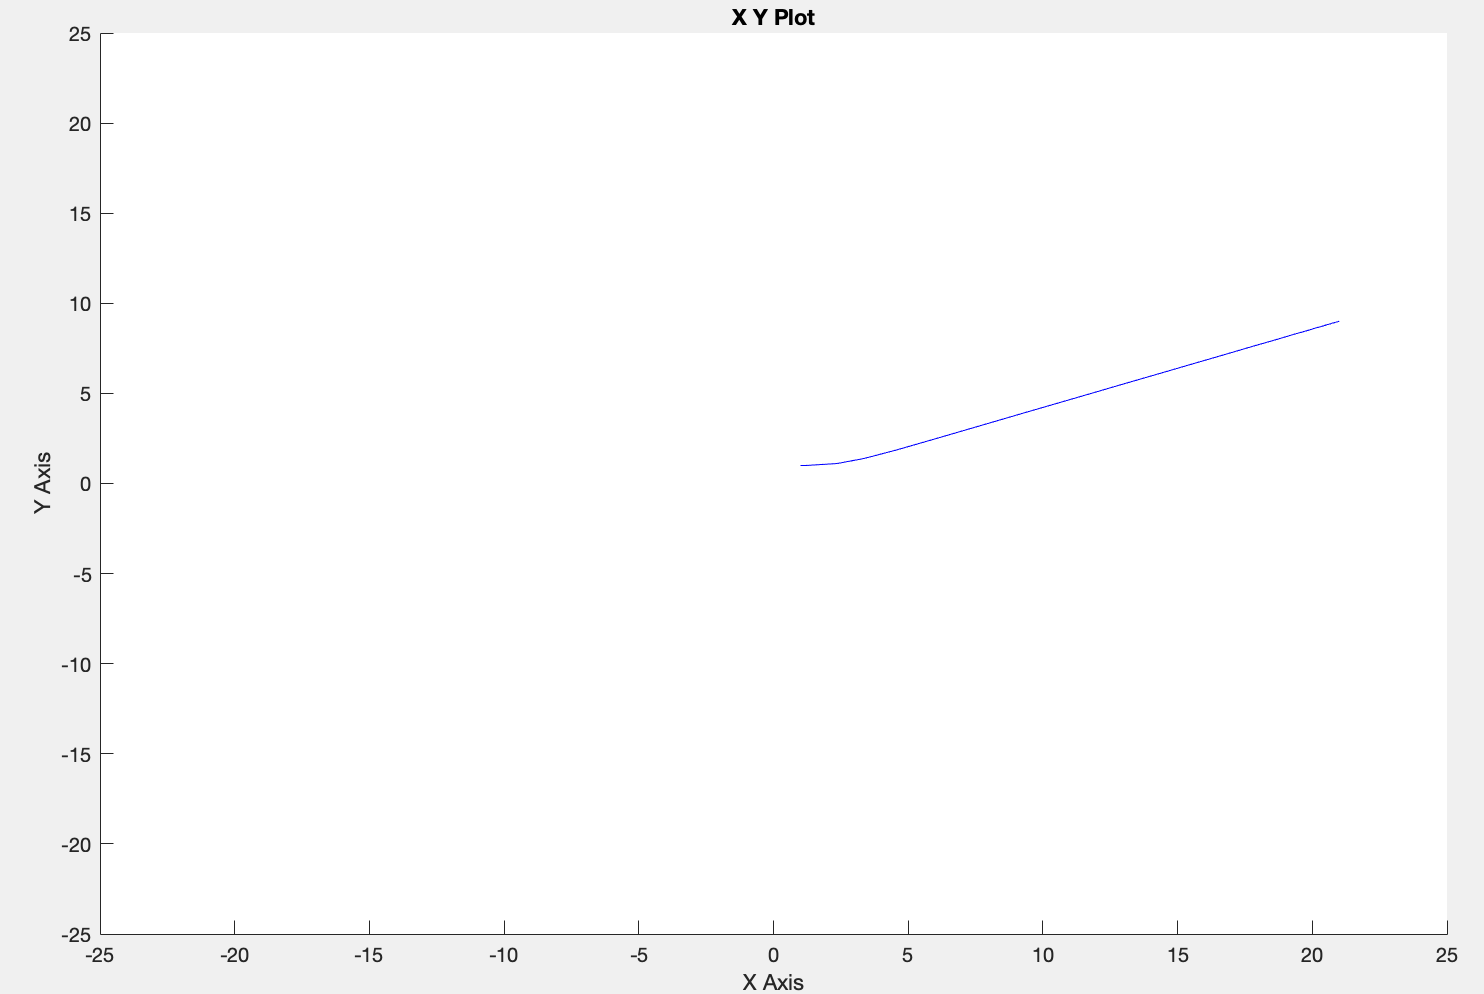
\includegraphics[scale=0.2]{xy_11.png}
				\end{minipage}
			}
			\caption{Кинетические (a) и фазовый (b) портреты при начальном значении $(x_0,y_0)=(1,1)$}
		\end{figure}
		\begin{figure}[htbp!]
			\centering
			\subfigure[$x(t),y(t)$]
			{
				\begin{minipage}[b]{.3\linewidth}
					\centering
					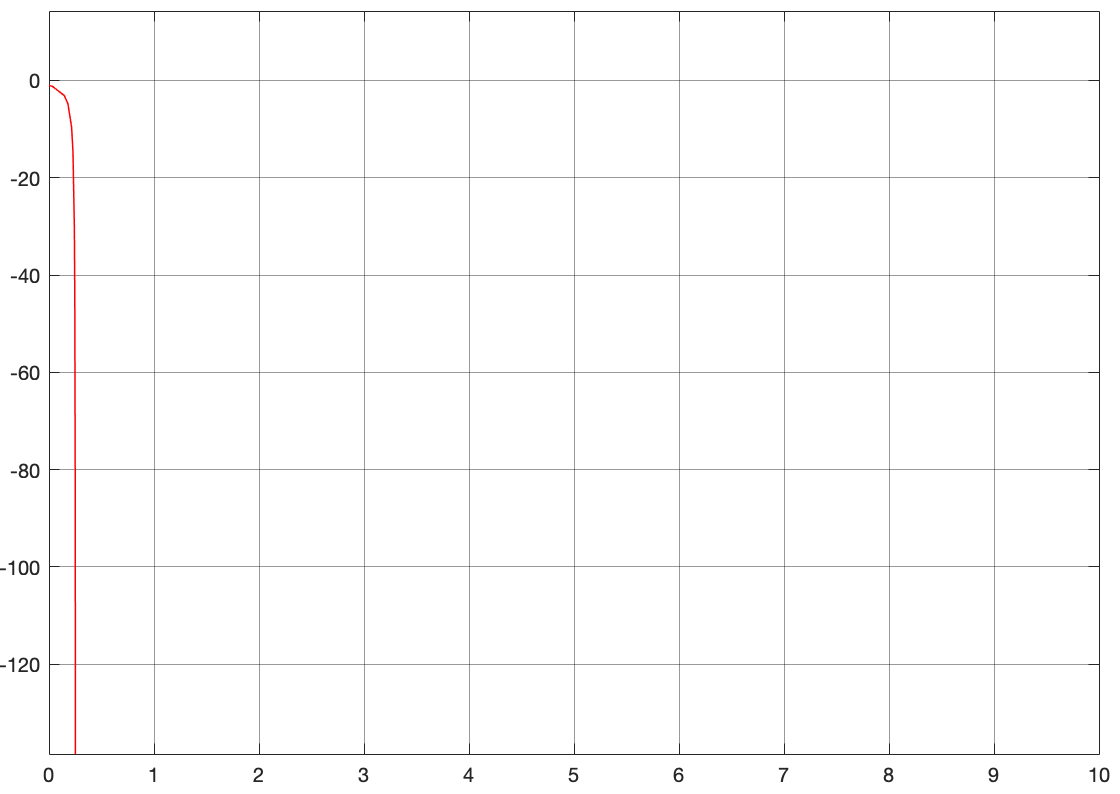
\includegraphics[scale=0.1]{x_2_-11.png}
				\end{minipage}
				\begin{minipage}[b]{.3\linewidth}
					\centering
					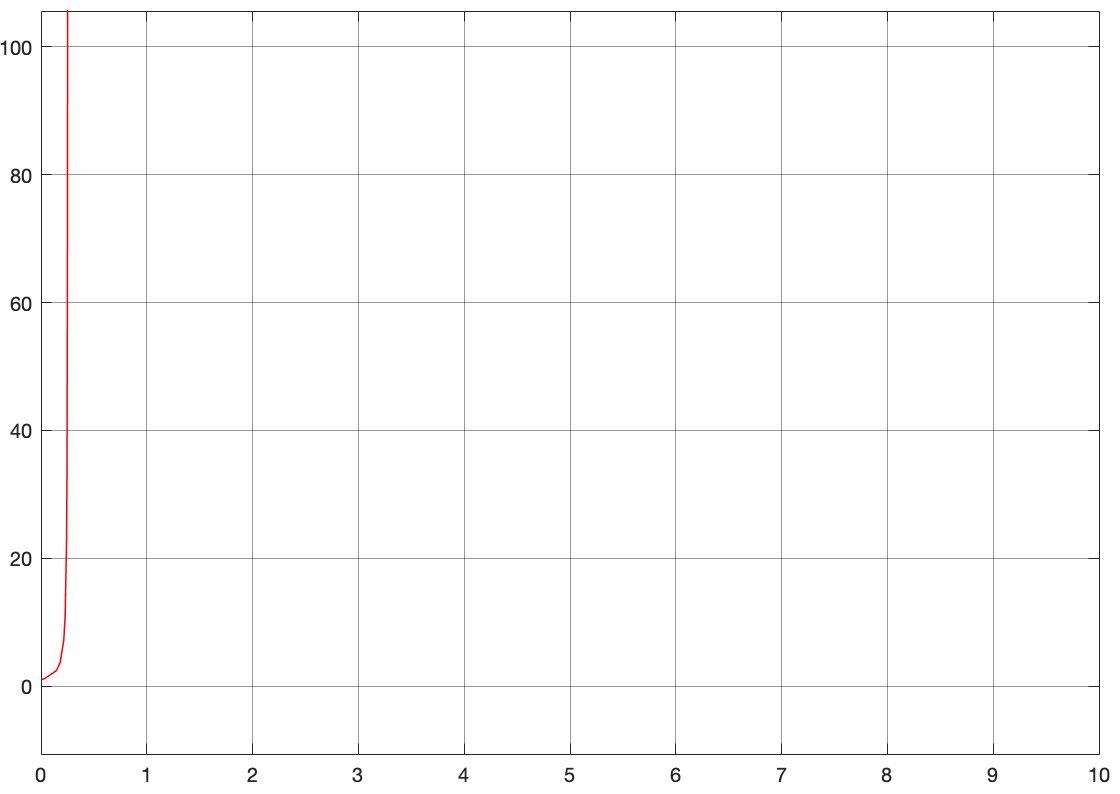
\includegraphics[scale=0.1]{y_2_-11.png}
				\end{minipage}
			}
			\subfigure[]
			{
				\begin{minipage}[b]{.3\linewidth}
					\centering
					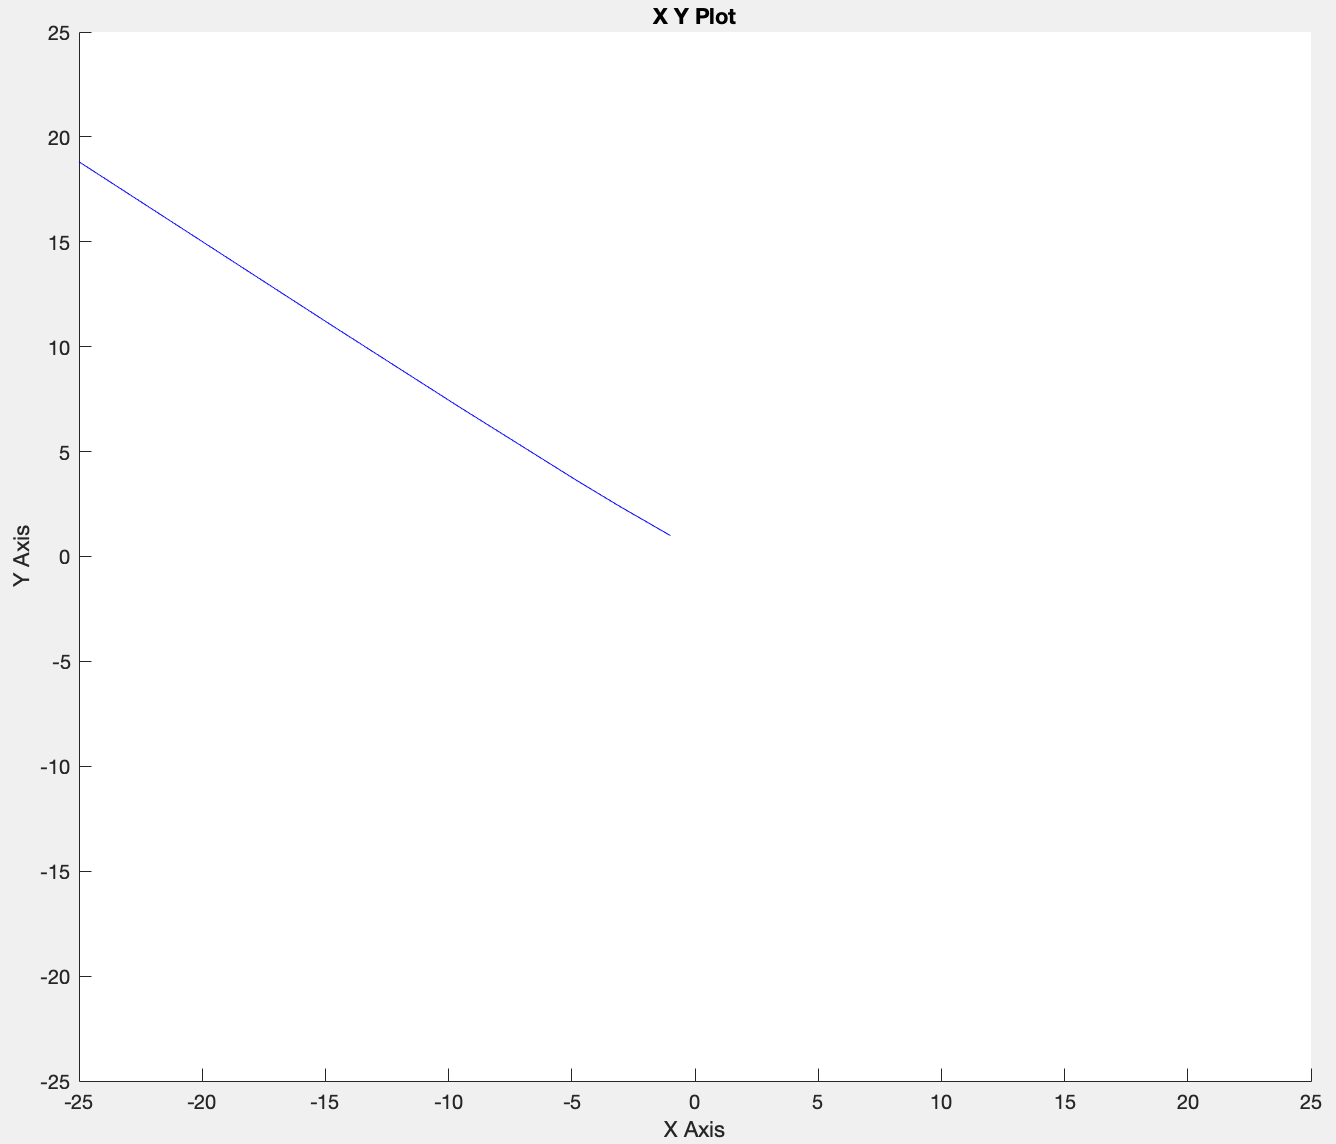
\includegraphics[scale=0.2]{xy_2_-11.png}
				\end{minipage}
			}
			\caption{Кинетические (a) и фазовый (b) портреты при начальном значении $(x_0,y_0)=(-1,1)$}
		\end{figure}
		\begin{figure}[htbp!]
			\centering
			\subfigure[$x(t),y(t)$]
			{
				\begin{minipage}[b]{.3\linewidth}
					\centering
					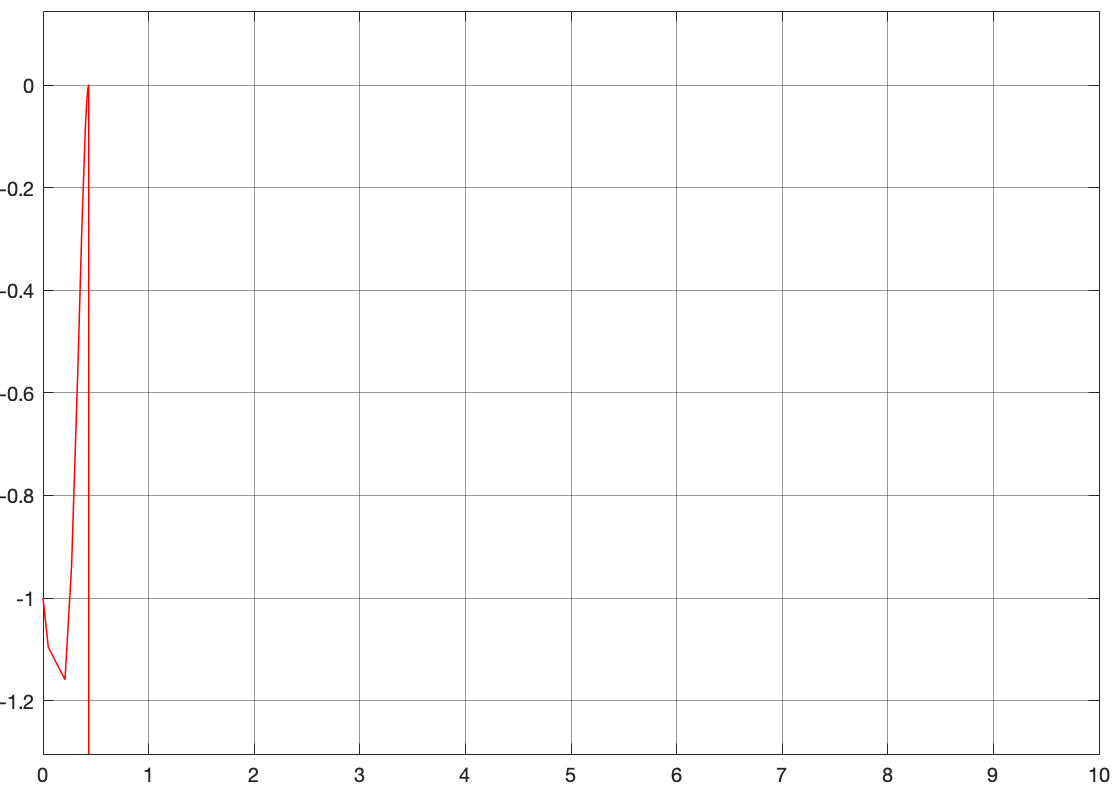
\includegraphics[scale=0.1]{x_2_-1-1.png}
				\end{minipage}
				\begin{minipage}[b]{.3\linewidth}
					\centering
					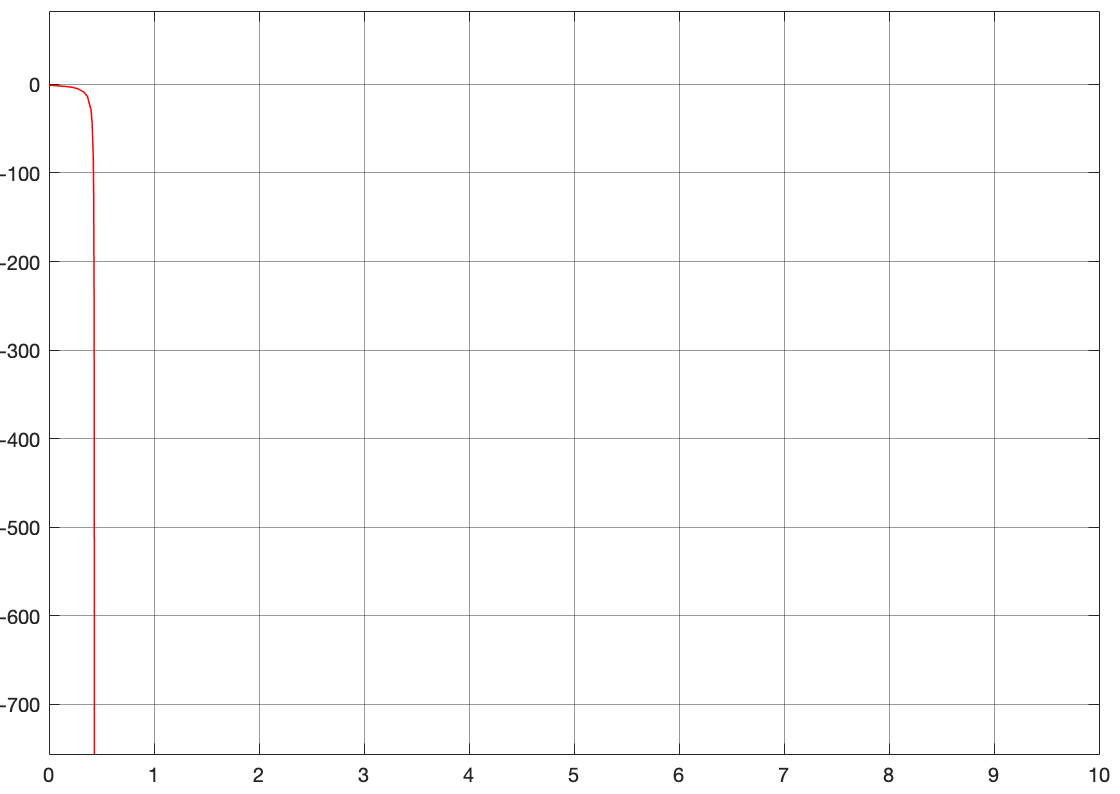
\includegraphics[scale=0.1]{y_2_-1-1.png}
				\end{minipage}
			}
			\subfigure[]
			{
				\begin{minipage}[b]{.3\linewidth}
					\centering
					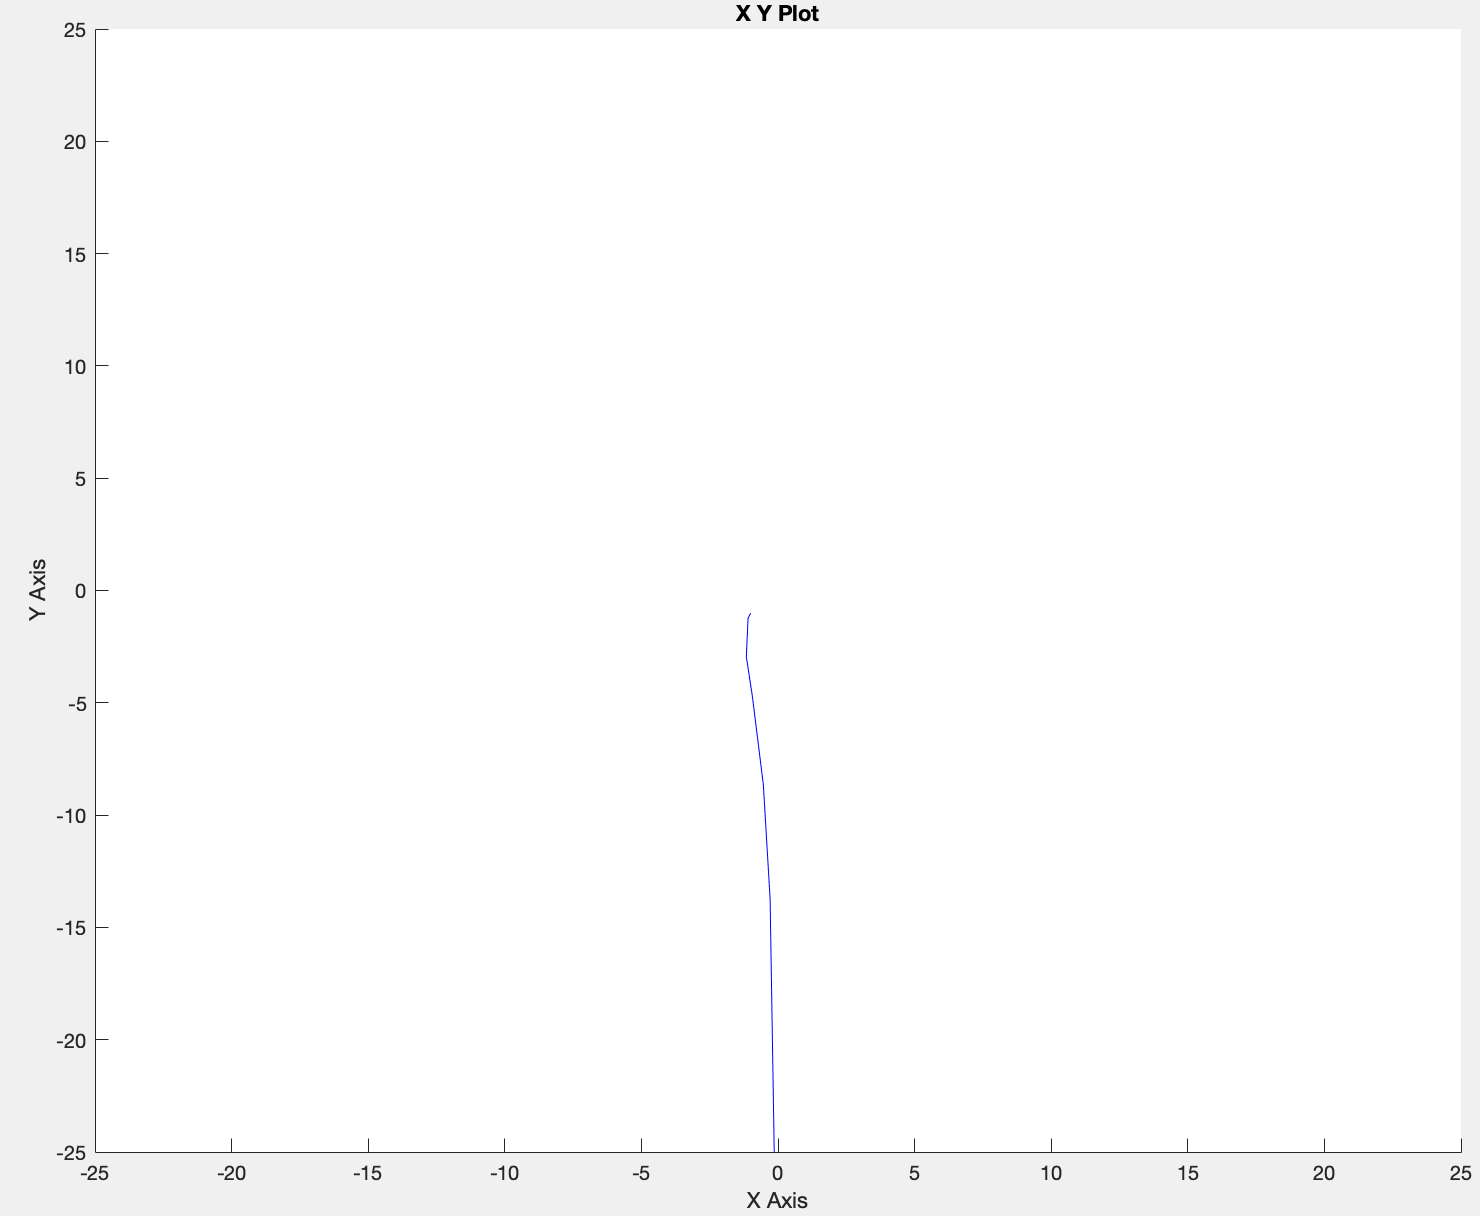
\includegraphics[scale=0.2]{xy_2_-1-1.png}
				\end{minipage}
			}
			\caption{Кинетические (a) и фазовый (b) портреты при начальном значении $(x_0,y_0)=(-1,-1)$}
		\end{figure}
		\begin{figure}[h!]
			\centering
			\subfigure[$x(t),y(t)$]
			{
				\begin{minipage}[b]{.3\linewidth}
					\centering
					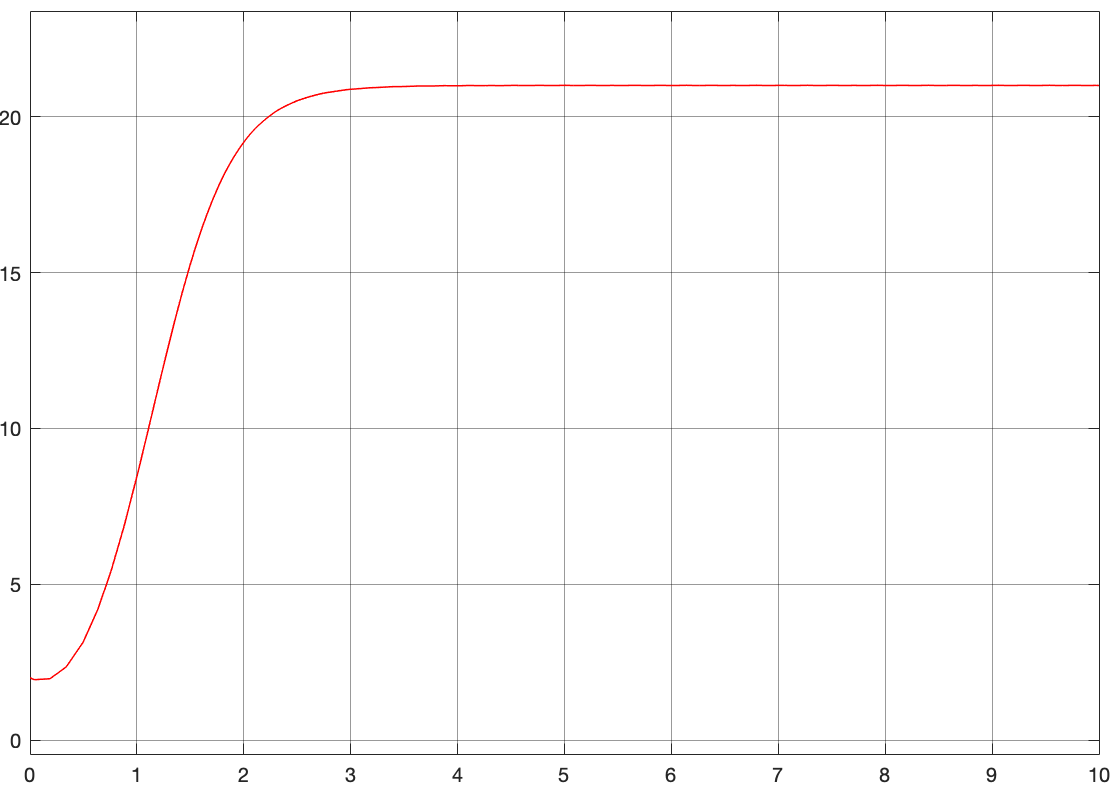
\includegraphics[scale=0.1]{x_2_1-1.png}
				\end{minipage}
				\begin{minipage}[b]{.3\linewidth}
					\centering
					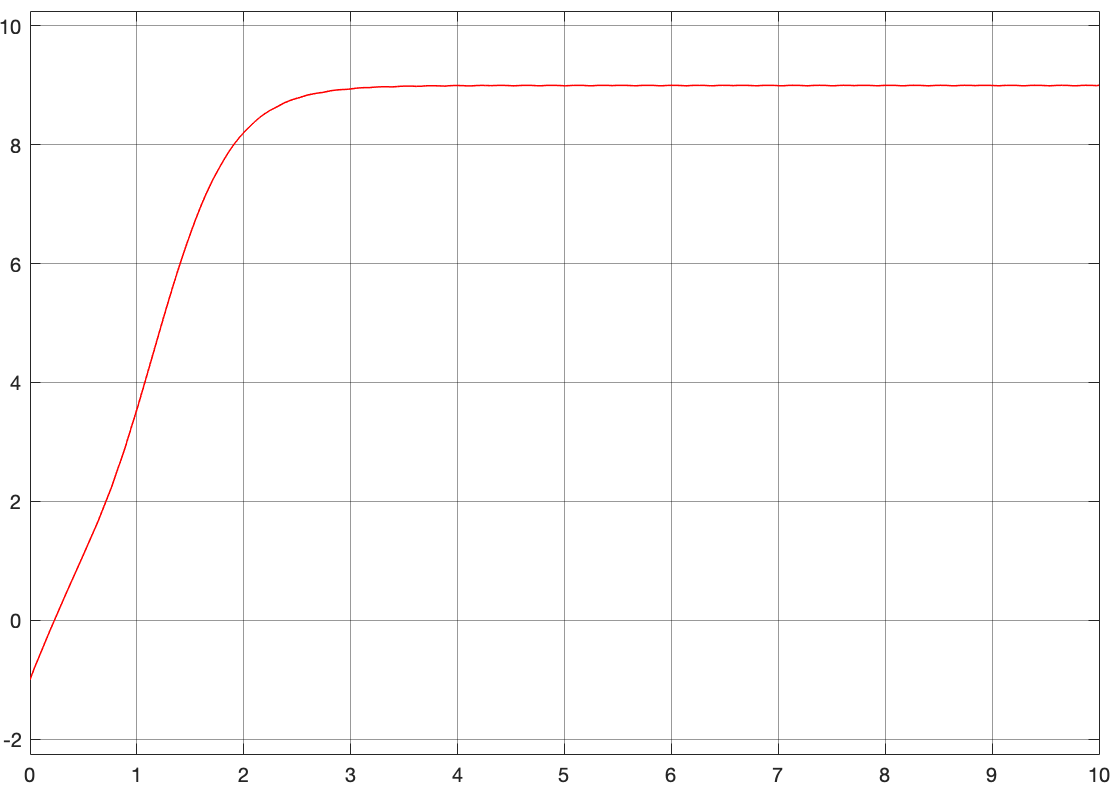
\includegraphics[scale=0.1]{y_2_1-1.png}
				\end{minipage}
			}
			\subfigure[]
			{
				\begin{minipage}[b]{.3\linewidth}
					\centering
					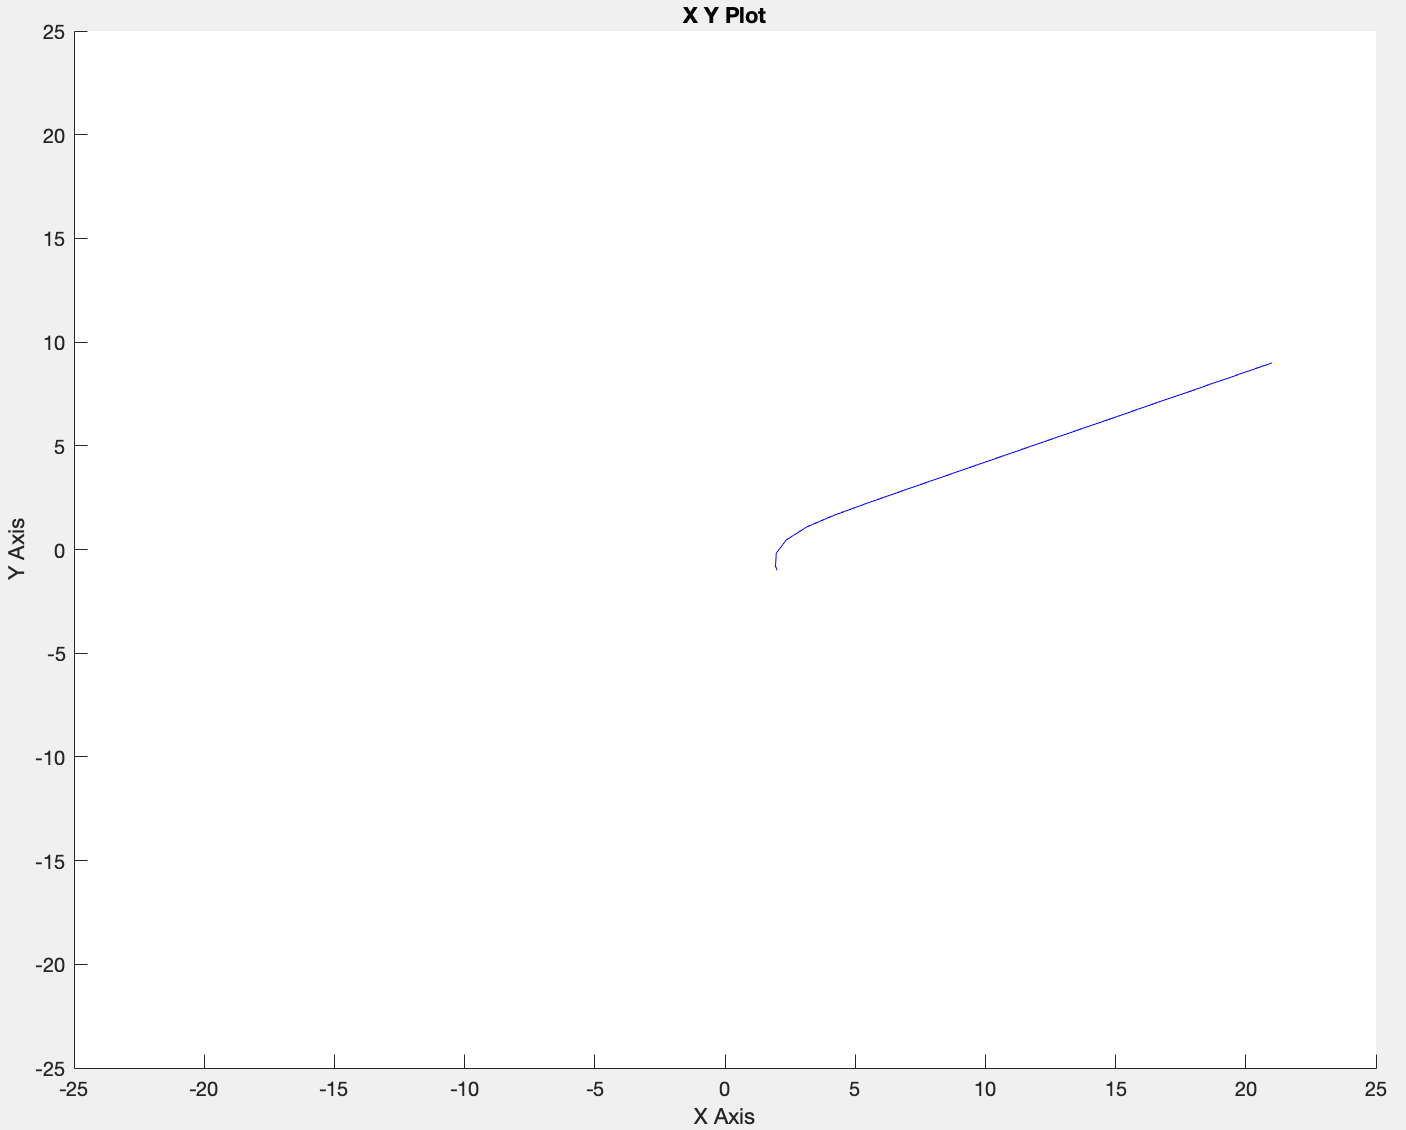
\includegraphics[scale=0.2]{xy_2_1-1.png}
				\end{minipage}
			}
			\caption{Кинетические (a) и фазовый (b) портреты при начальном значении $(x_0,y_0)=(1,-1)$}
		\end{figure}
		\begin{figure}[h!]
 		\center{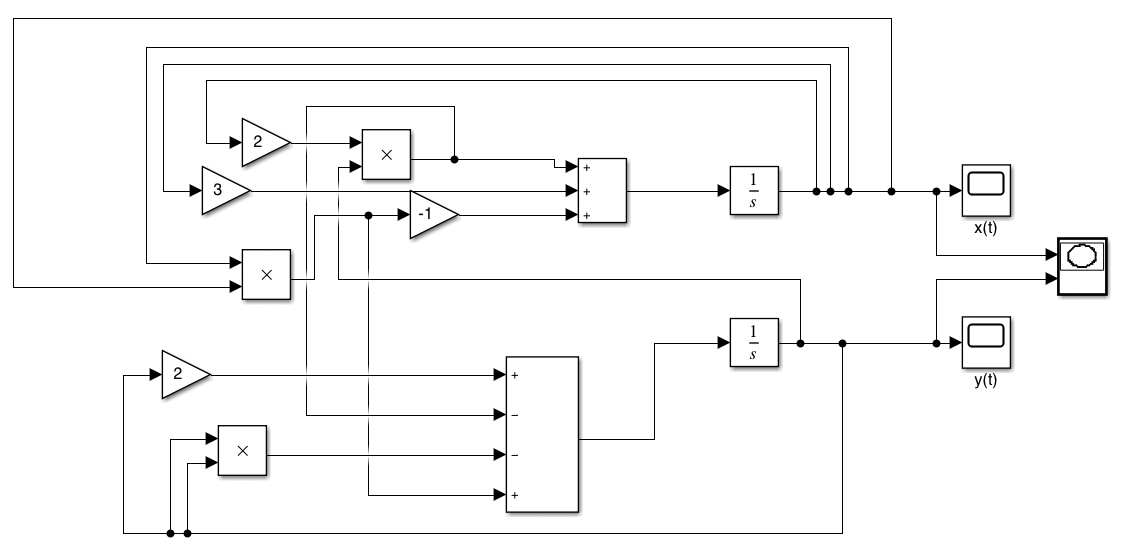
\includegraphics[scale=0.5]{model2.png}}
		\caption{Схема модели системы уравнений}
		\label{fig:image2}
		\end{figure}
		$$ $$
		$$ $$
		$$ $$
		\item Составим уравнения и опишем используемые константы:
		$$ \begin{cases}
			\frac{dE}{dt} = \frac{a_1SE}{N}+\frac{a_2SI}{N}+\frac{a_3SH}{N}-bE-kE\\
			\frac{dH}{dt} = cI-z_1fH-z_2dH-kH\\
			\frac{dS}{dt} = -\frac{a_1SE}{N}-\frac{a_1SE}{N}-\frac{a_1SE}{N}+(1-i)mN-kS\\
			\frac{dI}{dt} = bE-cI-gI-kI\\
			\frac{dR}{dt} = gI+z_2dH-kR+imN\\
			N = S+E+I+H+R
		\end{cases} $$
		
		$a_1/a_2/a_3=0.6/0.3/0.1$ -- коэффициент контакта в обществе/при симптомах/в больнице
		
		$y_1/y_2 = 0.01/0.99$ -- вероятность госпитализации/выздороветь
		
		$z_1/z_2 = 0.001/0.99$ -- вероятность умереть/выздороветь при госпитализации
		
		$m/k/N$ -- рождаемость/смертность/население в Уфе
		
		$\frac{1}{b}=15$ -- инкубационный период
		
		$\frac{1}{c}=10$ -- время до госпитализации
		
		$\frac{1}{g}=7$ -- время до выздоровления
		
		$\frac{1}{f}=20$ -- время до смерти
		
		$\frac{1}{d}=10$ -- время от госпитализации до выздоровления
		
		Пусть начальные значение это число вакцинированных $95\%, R=1045000, S=54000, E=1000$ 
		\begin{figure}[h]
			\center{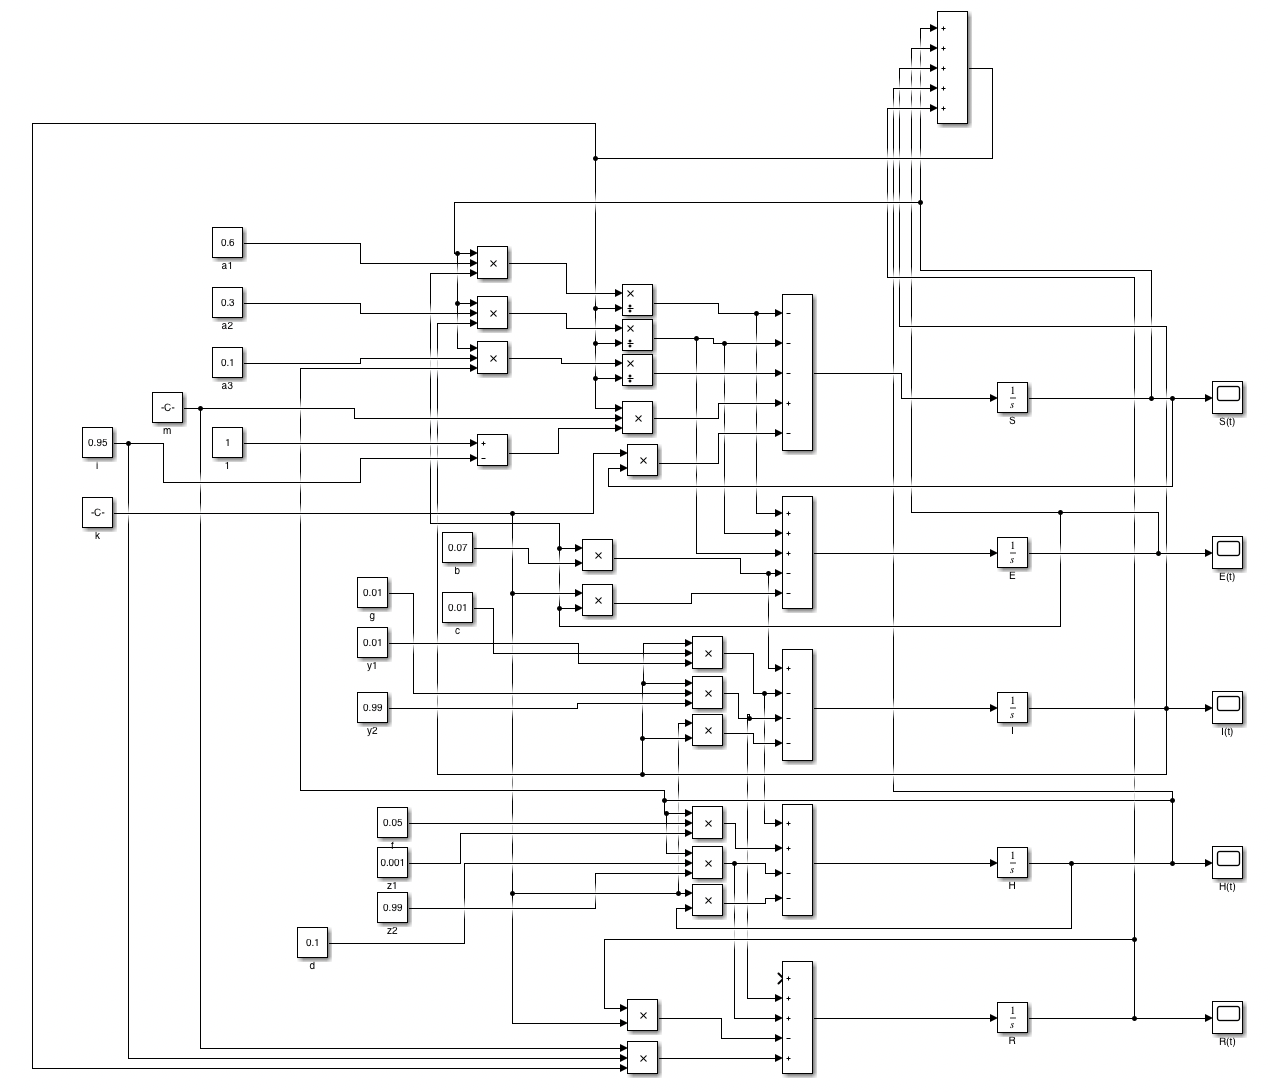
\includegraphics[scale=0.5]{model3.png}}
			\caption{Схема модели системы уравнений}
			\label{fig:image3}
		\end{figure}
		 
		 Как можно убедиться из графиков далее, в связи с очень высокой заболеваемостью число заболевший будет сначало очень сильно расти, но так вероятность умереть очень маленькая, то умирать люди почти не будут от ветрянной оспы.
		 \begin{figure}[h]
		 	\center{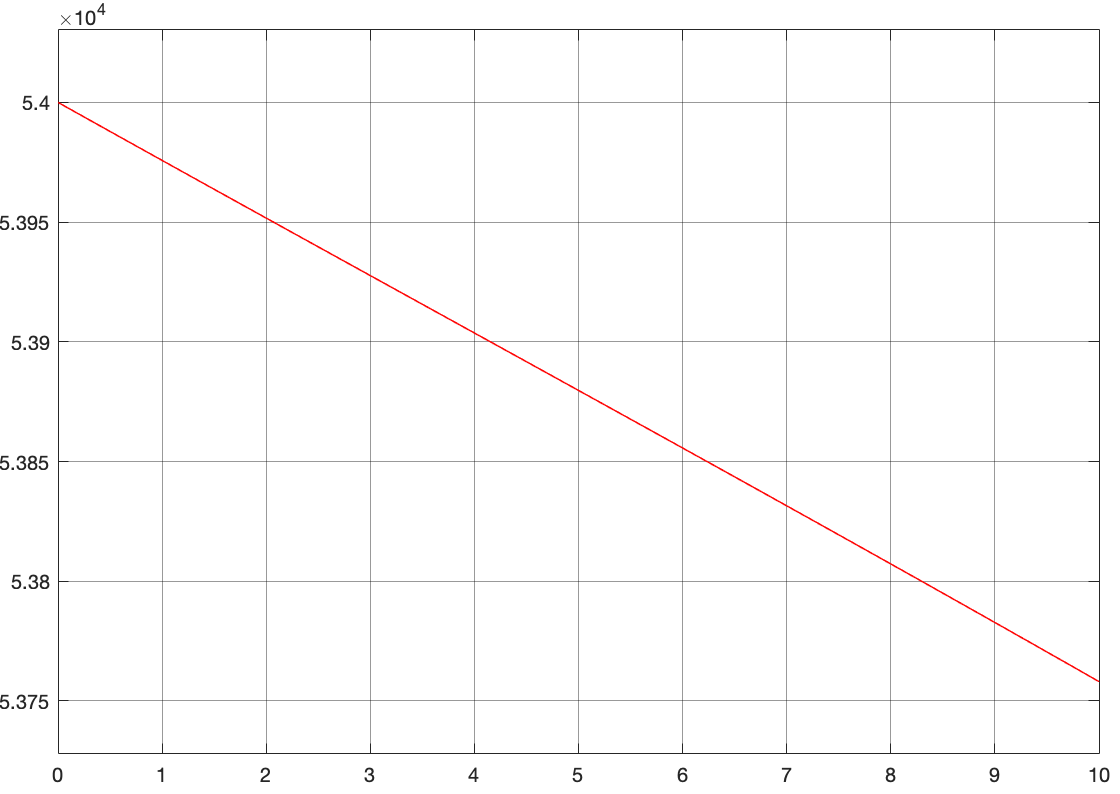
\includegraphics[scale=0.3]{S1.png}}
		 	\caption{S(t)}
		 	\label{fig:image4}
		 \end{figure}
	 \begin{figure}[h]
	 	\center{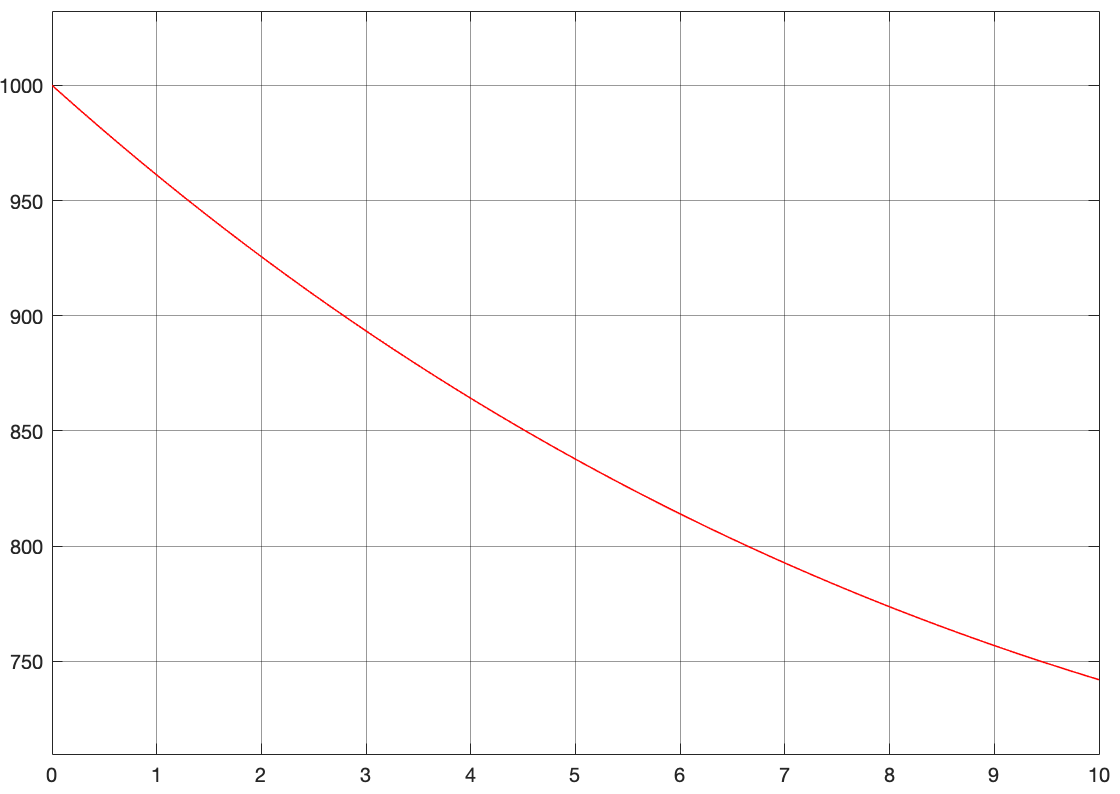
\includegraphics[scale=0.3]{E1.png}}
	 	\caption{E(t)}
	 	\label{fig:image5}
	 \end{figure}
 \begin{figure}[h]
 	\center{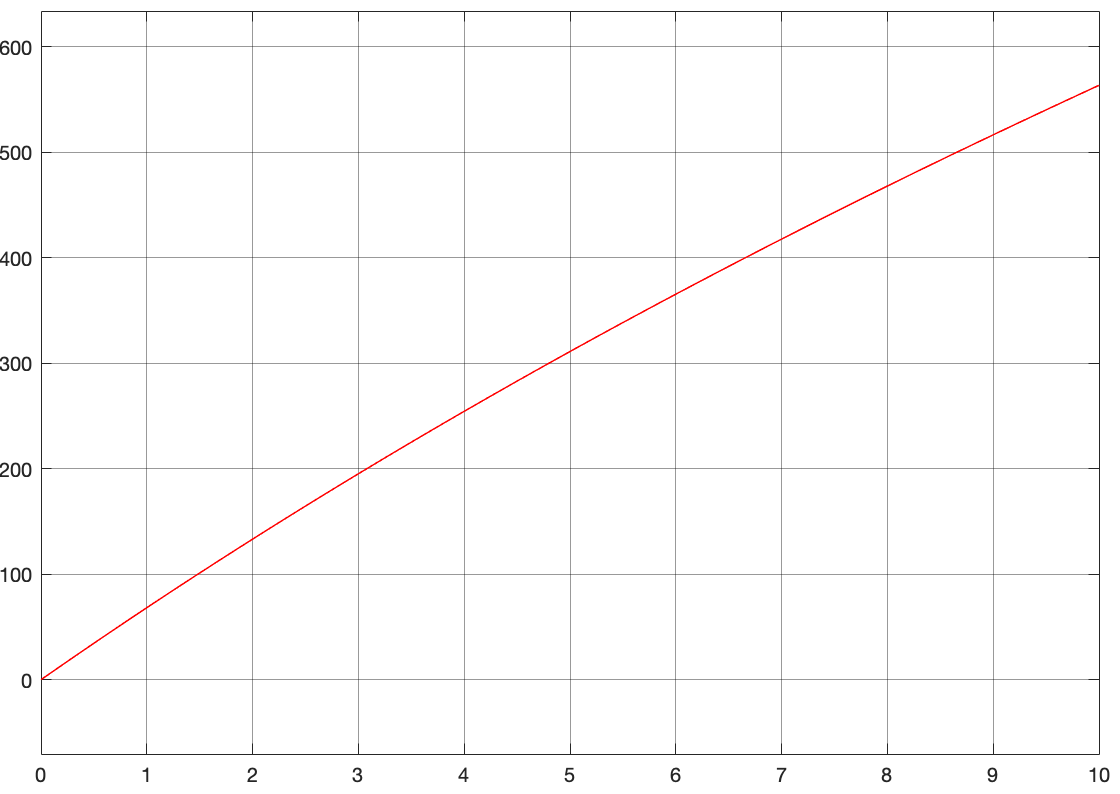
\includegraphics[scale=0.3]{I1.png}}
 	\caption{I(t)}
 	\label{fig:image6}
 \end{figure}
\begin{figure}[h]
	\center{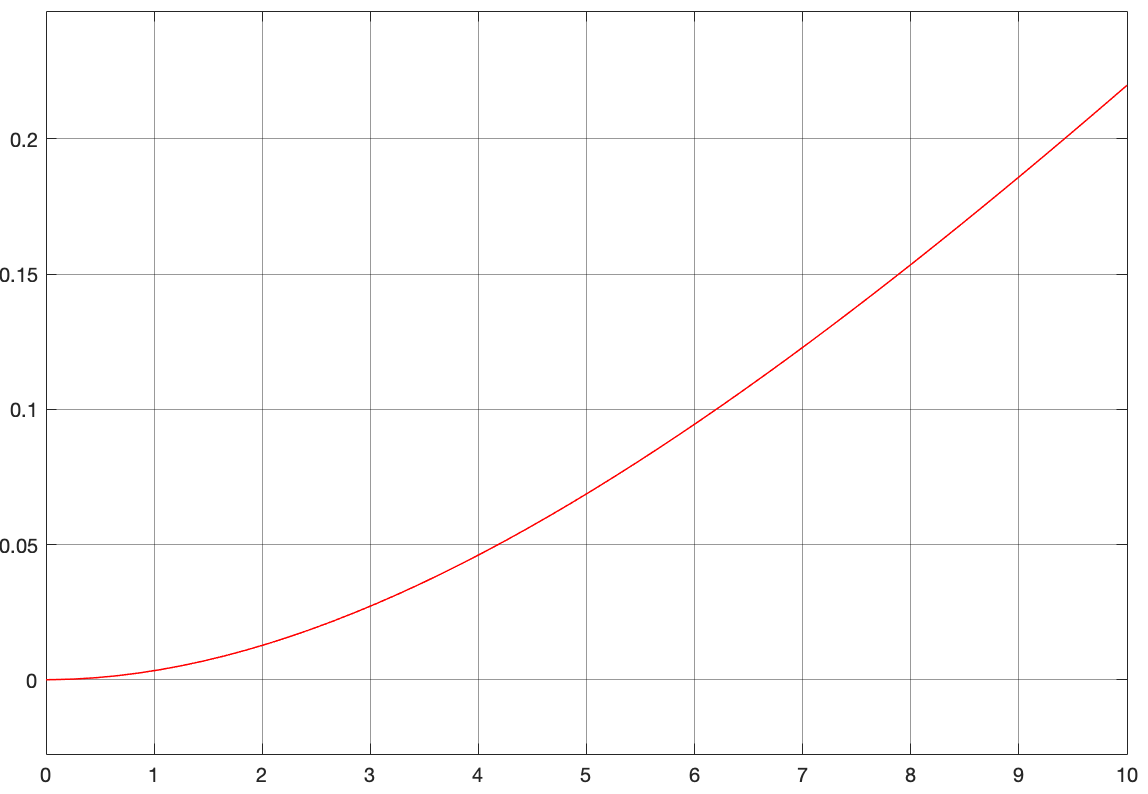
\includegraphics[scale=0.3]{H1.png}}
	\caption{H(t)}
	\label{fig:image7}
\end{figure}
\begin{figure}[ht]
	\center{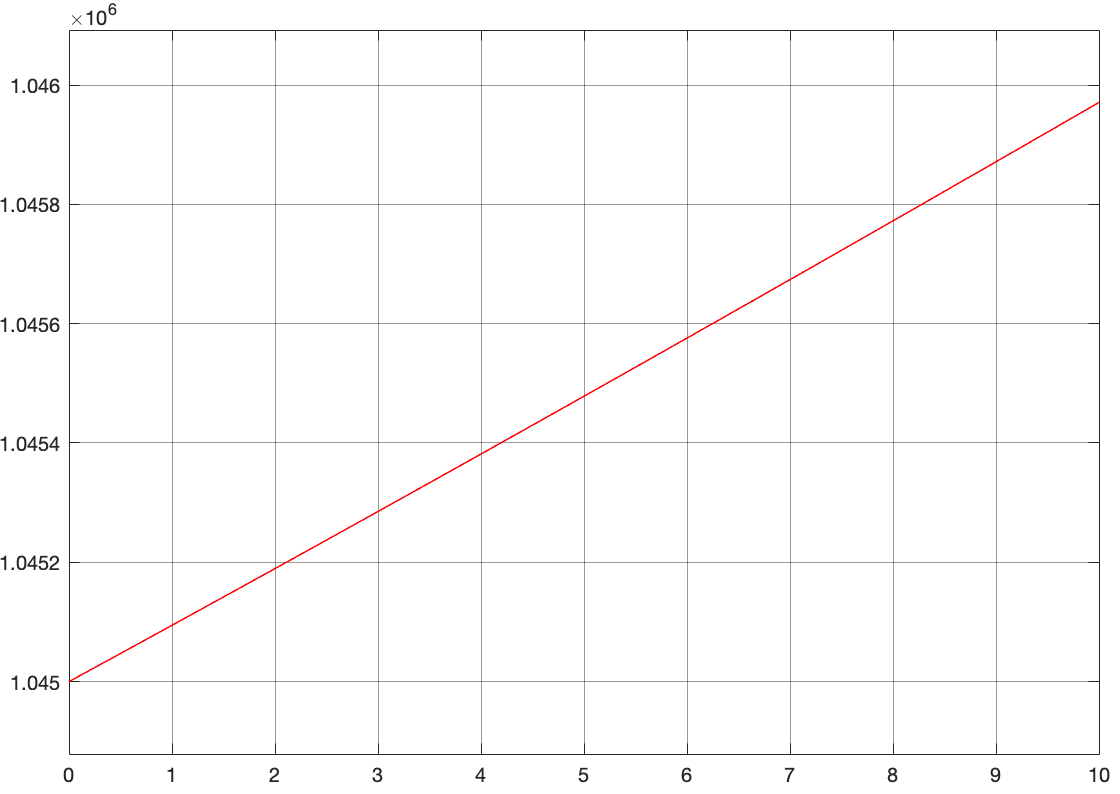
\includegraphics[scale=0.3]{R1.png}}
	\caption{R(t)}
	\label{fig:image8}
\end{figure}
	\end{enumerate}
\end{document}